\documentclass{article}

\usepackage{graphicx}
\usepackage{tikz}
\usepackage{tikzsymbols}
\usetikzlibrary{calc,patterns,shapes.geometric}
\pagestyle{empty}
\usepackage[margin=0pt]{geometry}
\geometry{papersize={14in,12in}}

\def\centerarc[#1](#2)(#3:#4:#5){\draw[#1] ($(#2)+({#5*cos(#3)},{#5*sin(#3)})$) arc (#3:#4:#5);}

\begin{document}
	\begin{figure}
		\centering
		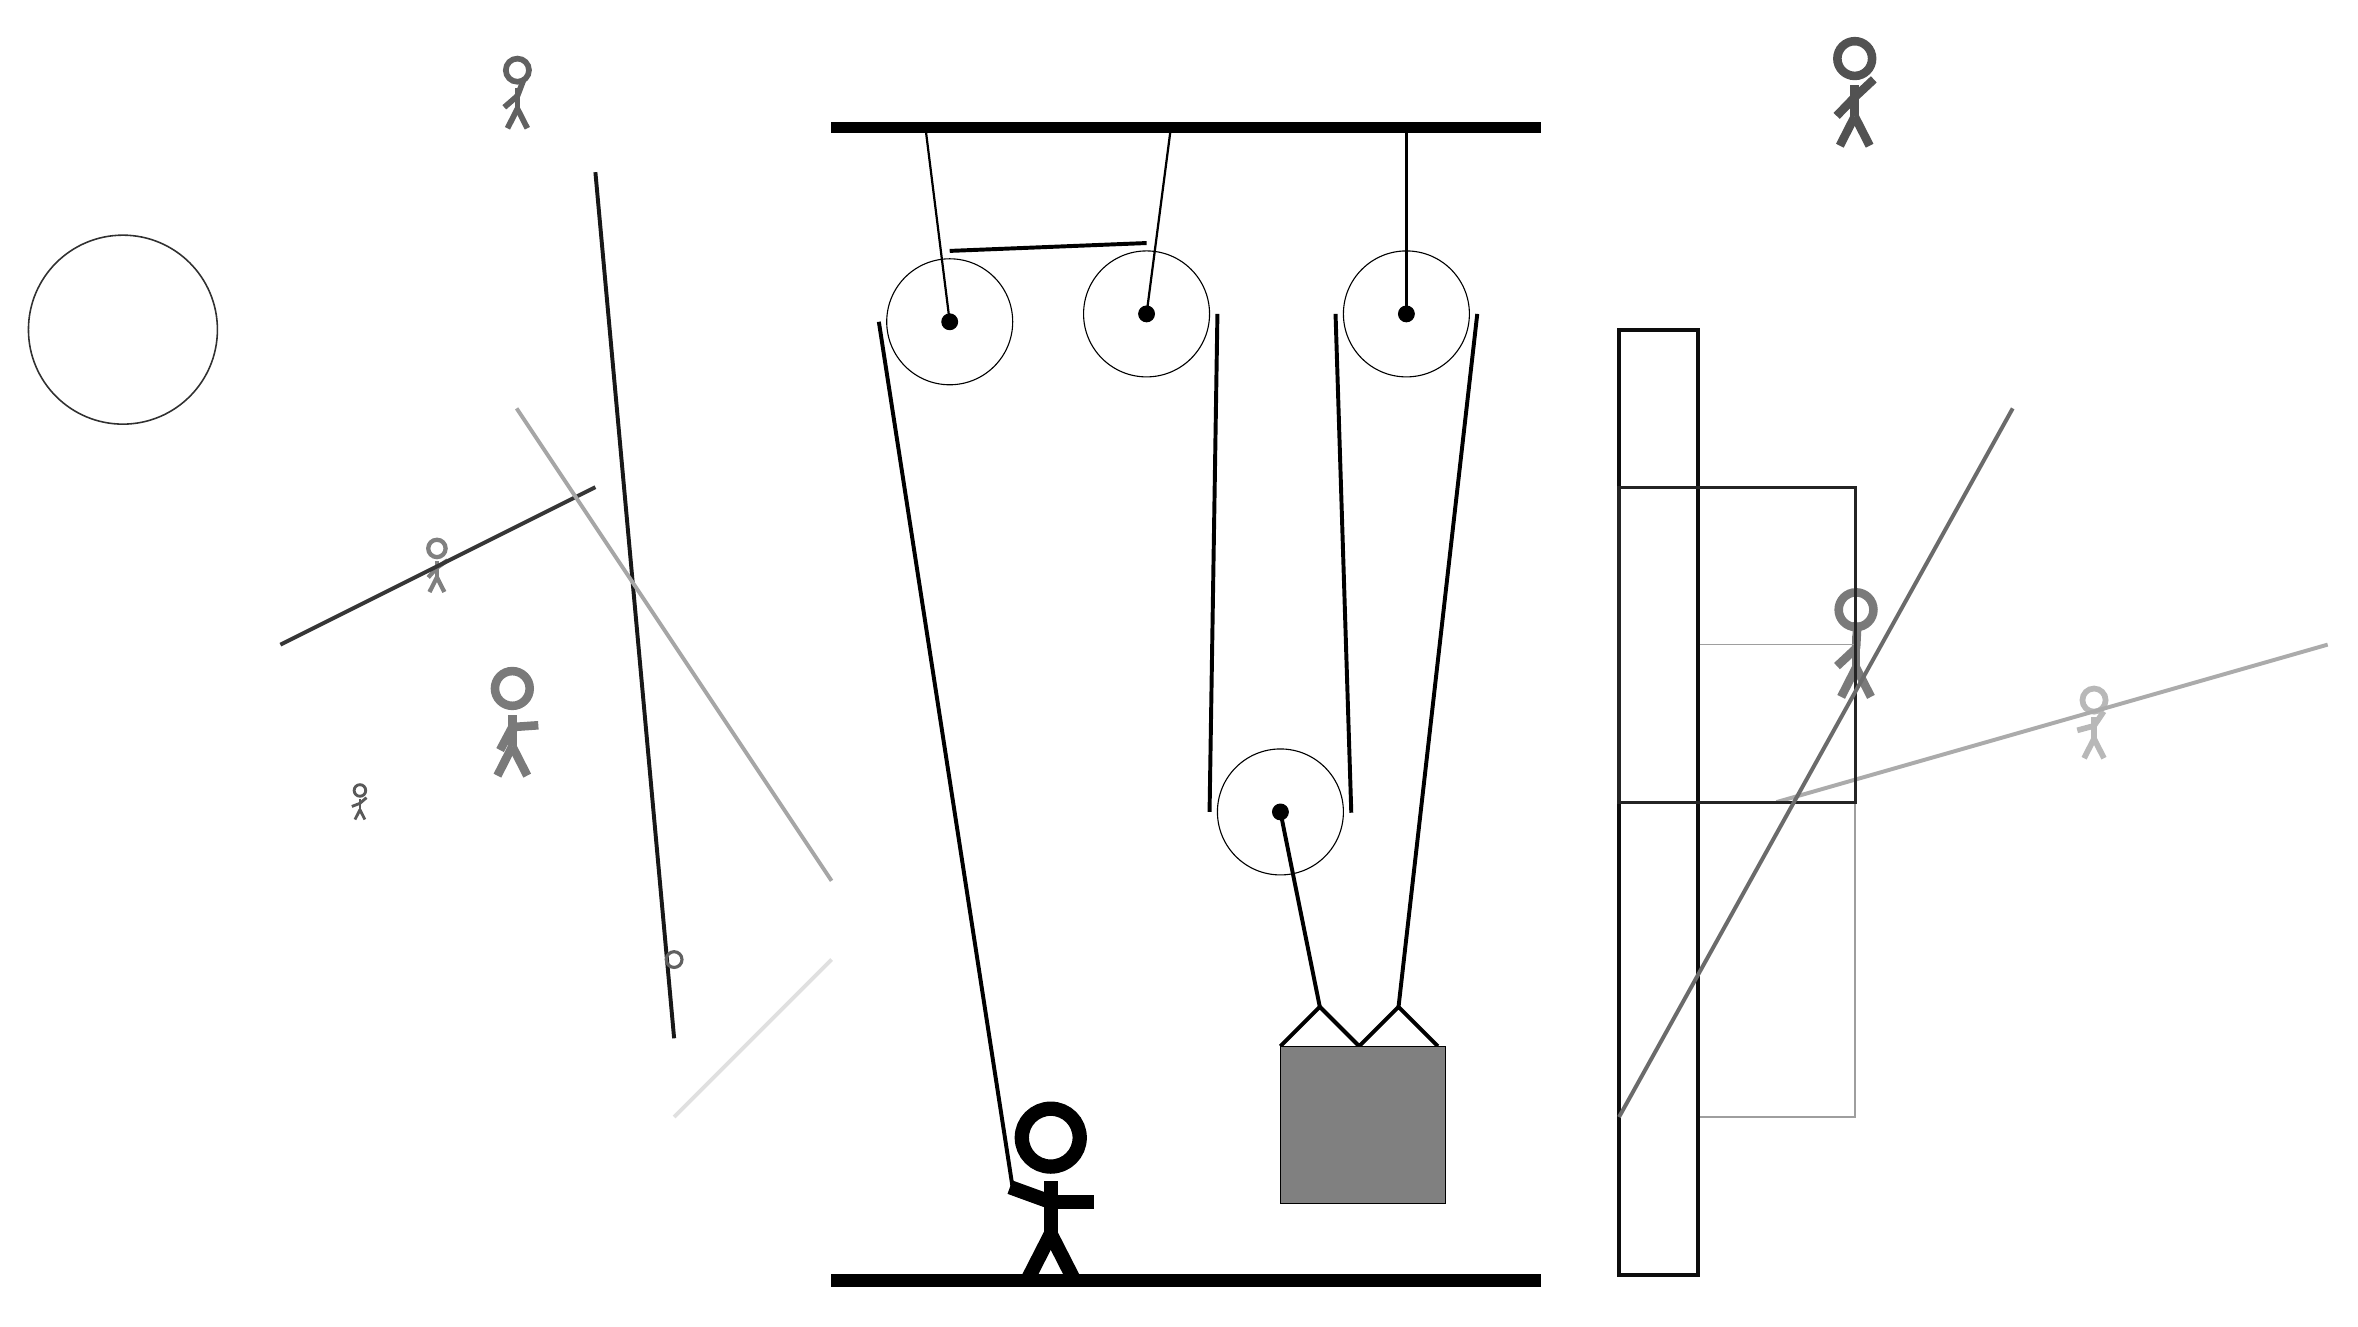
\begin{tikzpicture}
			%%%%% START %%%%%
			
			\draw[fill=black] (-3, 11.5) rectangle (6, 11.625);
			
			\draw (1, 9.2) circle (0.8);
			\draw[fill=black] (1, 9.2) circle (0.1);
			\draw[thick] (1, 9.2) -- (1.3, 11.5);
			
			\draw (4.3, 9.2) circle (0.8);
			\draw[fill=black] (4.3, 9.2) circle (0.1);
			\draw[thick] (4.3, 9.2) -- (4.3, 11.5);
			
			\draw (2.7, 2.875) circle (0.8);
			\draw[fill=black] (2.7, 2.875) circle (0.1);
			
			\node[line width=0.6mm, color=black!52] at (10, 5) {\Strichmaxerl[6][43][87]};
			
			\draw[line width=0.5mm, color=black!91](-5, 0) -- (-6, 11);
			\node[line width=0.6mm, color=black!50] at (-8, 6) {\Strichmaxerl[3][48][35]};
			\node[line width=0.4mm, color=black!68] at (10, 12) {\Strichmaxerl[6][46][43]};
			\draw[line width=0.5mm, color=black!79](-6, 7) -- (-10, 5);
			
			\draw[line width=0.2mm, color=black!38] (8, 5) rectangle (10, -1);
			\node[line width=0.6mm, color=black!28] at (13, 4) {\Strichmaxerl[4][15][56]};
			\draw [line width=0.5mm, color=black!90](6, 9) circle (0.0);
			\draw[line width=0.5mm, color=black!95] (7, 9) rectangle (8, -3);
			
			\draw[line width=0.5mm, color=black!33](9, 3) -- (16, 5);
			\draw[line width=0.4mm, color=black!86] (7, 3) rectangle (10, 7);
			\draw[line width=0.5mm, color=black!12](-5, -1) -- (-3, 1);
			\node[line width=0.7mm, color=black!52] at (-7, 4) {\Strichmaxerl[6][62][4]};
			\node[line width=0.6mm, color=black!62] at (-7, 12) {\Strichmaxerl[4][41][69]};
			\node[line width=0.7mm, color=black!65] at (-9, 3) {\Strichmaxerl[2][21][41]};
			\draw[line width=0.5mm, color=black!35](-3, 2) -- (-7, 8);
			\draw [line width=0.2mm, color=black!81](-12, 9) circle (1.2);
			
			\draw [line width=0.4mm, color=black!62](-5, 1) circle (0.1);
			\draw[line width=0.5mm, color=black!58](7, -1) -- (12, 8);
			
			\draw[line width=0.5mm]  (2.7, -0.1) -- (3.2, 0.4) -- (3.7, -0.1) -- (4.2, 0.4) -- (4.7, -0.1);
			\draw[fill=black!50] (2.7, -0.1) rectangle (4.8, -2.1);
			
			\draw (-1.5, 9.1) circle (0.8);
			\draw[fill=black] (-1.5, 9.1) circle (0.1);
			\draw[thick] (-1.5, 9.1) -- (-1.8, 11.5);
			
			\draw[line width=0.5mm](-0.7, -1.9) --  (-2.4, 9.1);
			\centerarc[line width=0.5mm](-1.5, 9.1)(90:180:0.9);
			\draw[line width=0.5mm](-1.5, 10.0) -- (1, 10.1);
			\centerarc[line width=0.5mm](1, 9.2)(0:90:0.9);
			\draw[line width=0.5mm](1.9, 9.2) -- (1.8, 2.875);
			\centerarc[line width=0.5mm](2.7, 2.875)(180:370:0.9);
			\draw[line width=0.5mm] (3.6, 2.865) -- (3.4, 9.2);
			\centerarc[line width=0.5mm](4.3, 9.2)(0:180:0.9);
			\draw[line width=0.5mm](4.2, 0.4) -- (5.2, 9.2);
			\draw[line width=0.5mm] (3.2, 0.4) -- (2.7, 2.875);
			
			\node at (-0.2, -2) {\Strichmaxerl[10][-20][0]};
			
			\draw[fill=black] (-3, -3) rectangle (6, -3.15);
			
			%%%%% END %%%%%
		\end{tikzpicture}
	\end{figure}	
\end{document}